\documentclass{article}
\usepackage{amsmath}
\usepackage{graphicx}
\usepackage[a4paper, margin=1in]{geometry}
\usepackage{pgfplots}
\pgfplotsset{compat=1.17}
\usepackage{afterpage}
\usepackage{float}

\title{k-Nearest Neighbors (k-NN) Implementation in Parallel}
\author{Epameinondas Bakoulas and Maria Sotiria Kostomanolaki}
\date{November 2024}

\begin{document}

\maketitle

\begin{abstract}
    This document explains the implementation of the \textbf{k-Nearest Neighbors (kNN)} algorithm in C, both in serial and parallel execution.
    The focus will mainly be on the parallel execution using threads to improve the speed of the execution, assuming that $C=Q$, the
    number of points in the dataset is in the millions and the number of dimensions is in the hundreds.
\end{abstract}

\section{Distance calculation}
In a $d$-dimensional space, the \textbf{Euclidean distance matrix} $D$ between two datasets 
$C$ and $Q$ is calculated as: 
\[
D = \sqrt{C.^2 - 2 C Q^T + (Q.^2)^T}
\]
where $C$ is the \textbf{corpus} dataset with $m$ points and $d$ dimensions, and $Q$ is the \textbf{query} dataset with $n$ points and $d$ dimensions.
$C.^2$ and $Q.^2$ denote element-wise squaring of the matrices and summing along the columns.
The function that implements the above is called \texttt{computeDistances}.

\section{Sequential implementation}
The \texttt{kNNsearch} function finds the k-nearest neighbors for each point in the matrix $Q$.
First, it splits the $Q$ matrix into \emph{blocks} in order minimize memory usage.
Then, it calculates the distances between the points in each block and the points in the corpus matrix $C$.
Finally, it finds the k-nearest neighbors and their distances for each point in the block.

\section{Parallel implementation}
We will assume $C=Q$ from now on and we will aim to find an \emph{approximate} solution for the k-nearest neighbors problem
for large datasets (number of points in the millions, and dimensions between 3 and 1000).


\subsection{Initialization}
We first create a struct called \texttt{Neighbor} that holds an \emph{index} and a \emph{distance}.
The function \texttt{kNN} initializes an $n \times k$ array \texttt{nearestNeighbors} to store the nearest neighbors for each point.
Each element in this array is initialized with a distance of \emph{INFINITY} and an index of $-1$.

\subsection{Splitting data into blocks}
The data points are divided into \emph{blocks} randomly. The randomess is achieved with the helper 
function \texttt{shuffleIndices} that takes an array of indices and shuffles them randomly. The first $n / numBlocks$ 
points are assigned to the first block, the next $n / numBlocks$ points to the second block, and so on.

For example, consider the matrix 
\[
C = \begin{bmatrix}
0 & 1 \\
1 & 2 \\
2 & 3 \\
3 & 4 \\
4 & 5 \\
5 & 6 \\
6 & 7 \\
7 & 8 \\
8 & 9 \\
9 & 10 \\
10 & 11 \\
11 & 12 \\
12 & 13 \\
13 & 14 \\
14 & 15 \\
15 & 16
\end{bmatrix}
\]

one possible split into 4 blocks is:
\[
\text{Block 1} = \begin{bmatrix}
0 & 1 \\
5 & 6 \\
10 & 11 \\
15 & 16
\end{bmatrix}, \quad
\text{Block 2} = \begin{bmatrix}
2 & 3 \\
4 & 5 \\
12 & 13 \\
14 & 15
\end{bmatrix}, \quad
\text{Block 3} = \begin{bmatrix}
1 & 2 \\
7 & 8 \\
9 & 10 \\
13 & 14
\end{bmatrix}, \quad
\text{Block 4} = \begin{bmatrix}
3 & 4 \\
6 & 7 \\
8 & 9 \\
11 & 12
\end{bmatrix}
\]

\subsection{Processing blocks}
For each block, we calculate the distances between the points and update the nearest neighbors.
Finding the k-Nearest Neighbors is achieved with the function \texttt{quickSelect}. It takes as input
the neighbors of a point (an array of \texttt{Neighbor}s) and quick selects the distances to find the $k$ nearest neighbors.
The blocks are processed in parallel. Each thread processes a block, until all blocks are processed.

After processing blocks, the nearestNeighbors matrix (NN) will look like (only first 4 points are shown, $k=3$):
\[
\text{NN} = \begin{bmatrix}
(0, 0.0) & (5, 7.07) & (10, 14.14) \\
(1, 0.0) & (7, 8.49) & (9, 11.31) \\
(2, 0.0) & (4, 2.83) & (12, 14.14) \\
(3, 0.0) & (6, 4.24) & (8, 7.07) \\
\end{bmatrix}
\]

\subsection{Improving the Solution}
The solution is improved by finding distances between points in different blocks using a subset of the points. 
For example, if we combine pairs of blocks by choosing only $50\%$ of the points in random (2 points from each block),
we might get:
\[
\text{Subset from Block 1} = \begin{bmatrix}
0 & 1 \\
10 & 11
\end{bmatrix}, \quad
\text{Subset from Block 2} = \begin{bmatrix}
2 & 3 \\
14 & 15
\end{bmatrix}
\]
We'll calculate the distance matrix using these points to update their neighbors. In the above example, we will find the
distance between the points $[0, 1]$, $[2, 3]$, $[10, 11]$ and $[14, 15]$ and update their nearest neighbors if we end up finding a new
nearest neighbor.

After this improvement, the nearestNeighbors matrix (NN) will look like:
\[
\text{NN} = \begin{bmatrix}
(0, 0.0) & (5, 7.07) & (2, 2.83) \\
(1, 0.0) & (7, 8.49) & (9, 11.31) \\
(2, 0.0) & (4, 2.83) & (0, 2.83) \\
(3, 0.0) & (6, 4.24) & (8, 7.07) \\
\end{bmatrix}
\]

The block pairs are processed in parallel. Each thread processes a pair of blocks, until all pairs are processed.
If we process the pair $(i, j)$, we do not have to process the pair $(j, i)$, since the distances are symmetric.

\subsection{Analyzing the end results}
The last step is to find the \emph{Recall} and \emph{Queries per second} of the algorithm. Recall is equal to the percentage of the
correct neighbors that we find. It is calculated by comparing the ground truth (exact) solution of the algorithm with the 
approximate solution.
\[
\text{Recall} = \frac{\text{\# correct neighbors}}{\text{total neighbors}}
\]
Queries per second is the number of queries that the algorithm processes in one second. 
\[
\text{Queries per second} = \frac{\text{\# points}}{\text{execution time (seconds)}}
\]


\section{Benchmarks}
We will display the benchmarks produced from testing the data \emph{sift-128-euclidean}.
It has a total of $n=1,000,000$ points and $d=128$ dimensions, and we'll find the $k=100$ nearest neighbors.
Tested on a computer with CPU: i5-11400F (6 cores, 12 threads), 16GB RAM, and OS: Linux Mint 22.
The following graph summarizes the benchmarks for different implementations:

\begin{figure}[H]
\centering
\begin{tikzpicture}
    \begin{axis}[
        title={Recall-Queries per second tradeoff - up and to the right is better},
        xlabel={Recall (\%)},
        ylabel={Queries per second},
        legend pos=north east,
        ymajorgrids=true,
        grid style=dashed,
        yticklabel style={/pgf/number format/fixed},
        scaled y ticks=false,
        width=0.9\textwidth,
        height=0.3\textheight,
        ymode=log,
    ]

\addplot[
    color=blue,
    mark=square,
    ]
    coordinates {
    (2.22, 11995) (8.13, 2516) (25.34, 938) (57.36, 446)
    };
    \addlegendentry{Pthreads}

\addplot[
    color=red,
    mark=triangle,
    ]
    coordinates {
    (2.24, 12064) (8.12, 2504) (26.52, 905) (57.19, 460)
    };
    \addlegendentry{OpenMP}

\addplot[
    color=green,
    mark=o,
    ]
    coordinates {
    (2.24, 11846) (8.09, 2542) (26.54, 915) (57.29, 462)
    };
    \addlegendentry{OpenCilk}

\addplot[
    color=purple,
    mark=diamond,
    ]
    coordinates {
    (2.23, 4251) (8.08, 897) (26.39, 278) (57.21, 135)
    };
    \addlegendentry{Sequential}

\end{axis}
\end{tikzpicture}
\caption{Queries per second vs Recall for different implementations (4 threads)}
\end{figure}

All 3 parallel implementations produce very similar results. 
We can clearly see that the parallel implementations are much faster than the sequential one
by a factor of $\times2.8-3.4$ using 4 threads.

To measure the recall we used only the first 10000 points of the dataset and we did not take into account
the position of the neighbors in the \texttt{nearestNeighbors} array. We only checked if the neighbors were the same
with the results produced by Matlab's \texttt{knnsearch} function. The correctness of this approach is guranteed
by the fact that we introduced randomness in the algorithm, and also because n is very large.

What if we wanted to maximize the \emph{Recall} for this dataset using the same algorithm?
We tested it with OpenMP and the end results were Recall = $99.98\%$ and Queries per second = $241$.
This result beats the last sequential result (Recall = $57.21\%$, Queries per second = $135$) by a factor of $\times1.7$, 
both in Recall and Queries per second!

Can we do better? Yes we can, by increasing the number of threads. We tested the same dataset with 8 threads and the
results were slightly better, by a factor of $\times1.1-1.2$ in Queries per second. This is expected due to hardware
bottlenecks, but it does allow us to fully utilize the CPU.


\end{document}
